\Chapter{An Artist at Home}{Glyn Court}

Whatever its imperfections, our house is unquestionably individual, and (as my wife has hinted) this is because it was planned and, for the most part, actually built by one man, my father. As he saw it, the ideal house had little to do with architectural fashion or modernity but everything to do with the old values of village society and its craftsmen; and as so much of the old life was passing away, and he treasured the memories of the friends of his youth, he determined to preserve what he could by that workmanship of his which sprang from the soil of Somerset.

The old craftsmen had been compelled by poverty to use their materials with the most rigid economy; my father's generation, though they were beginning to live more amply, would never throw away a good nail or screw, never cut a knot in a length of string, never discard a length of timber; a cobbler - as I can remember from the war years - would juggle for long periods with a bend ox leather to find an extra sole or even an infilling for a cue. "Wicked waste" was a phrase often heard on their lips. Yet not only economy was at the root of this behaviour, but something deeper, a respect amounting to reverence - though they would not have consciously named it so - for the materials of their craft and love and intimate understanding of their qualities. It is traditionally in carpenters and wheelwrights, working with living individual material, that this attitude has always been most highly developed, and in this also my father ran true to the type, He loved all timber, I believe, but not uncritically, and he had his favourites. Nothing could arouse his enthusiasm like good honest English oak: he loved its hardy, workable close grain, its mellowness and dignity; he would caress it and lovingly feel its texture, but he would shake his head sadly over the Austrian oak of which more and more came in after 1900, easier to work, maybe, but it had not the character, the staying-power, the hardy grain of the true, well-seasoned native. Perhaps he saw a parable in it too. Besides, as he saw it, the true carpenter, if not the joiner, should in some measure make the dead tree live again, and to all the flat surfaces of the heavy oak in his house he gave a natural finish with saw and plane alone, and on the curves he left the marks of chisel and gouge, only slightly evened by sanding. "Here is good timber," he seemed to say, "let it be."

By the time he came to build his own house, however, the good timber of his youth was hardly to be found. During the Great War the hardwood forests had been mercilessly felled, the stocks of matured timber so carefully laid down over the years were exhausted, and were not being replaced.

In this dilemma the ingrained habits of economy came to his aid. As my wife has written elsewhere, he rescued beams and panels of oak from a rubbish heap, worked on them, and pieced them together to make doors; from a mill in his village which had just ceased to work he salvaged the mill wheel; out of the cross-pieces of this he fashioned the surround of his sitting room fireplace, in which the bolt holes are still visible; and he made his staircase, both treads and risers, out of the vanes.

\begin{figure}
	\centering
     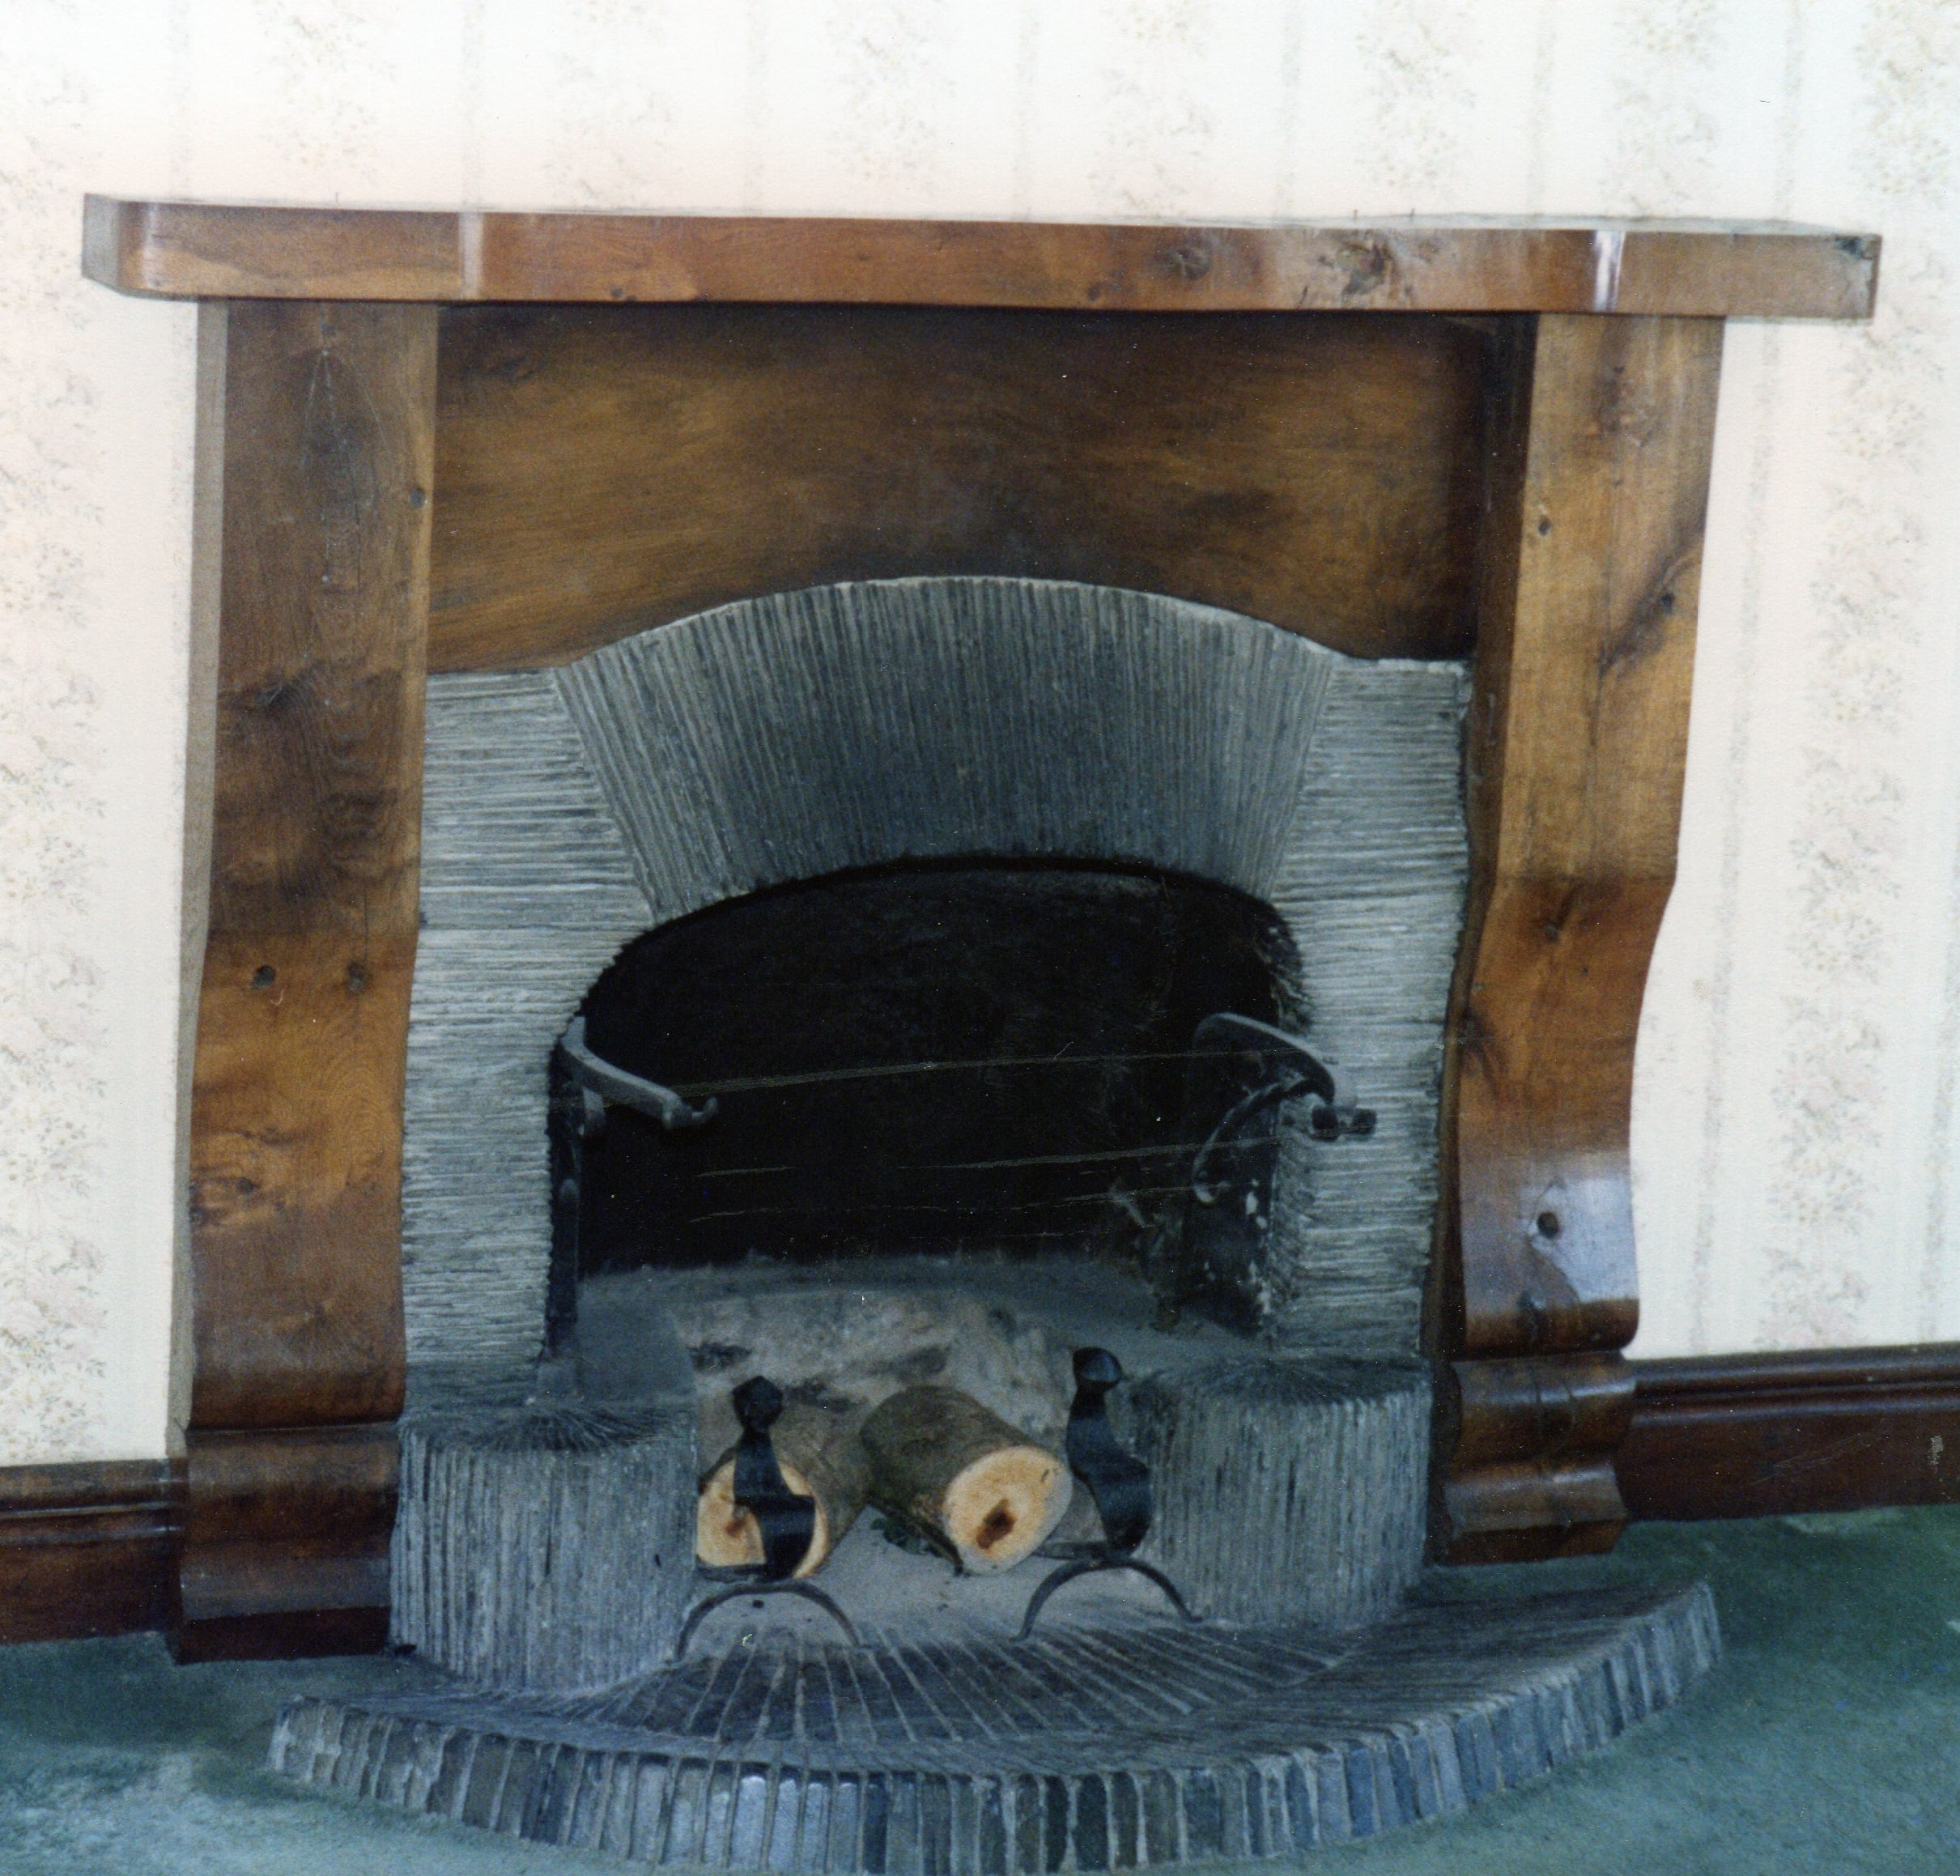
\includegraphics[width=1\textwidth]{figures/Fireplace}
     \caption{The fireplace, constructed by William Court using locally source Timber and Slate}
     \label{fig:Fireplace}
\end{figure}

It was, I believe, a matter of pride with him, not merely a result of straitened circumstances in the 1920s, that he should use local materials throughout his home. Very remarkably, using local resources, and working in a local tradition, he nevertheless built a house peculiar to himself and in some of its components, at least, quite unique.

Certainly his slate fireplace is unique. Slate seems an unlikely material, but my father had two good reasons: availability, and – better still - sentiment. The latter argument he never could resist.

Near Treborough, on the steep hillside two miles above Roadwater, is an abandoned slate quarry. It has long been deserted; the last two regular workmen, Eli Vickery and his son, ceased in the late 1930's; but in my father's youth it provided employment for thirty men. Father was determined to have a capacious fireplace in his best room, and one built naturally of local materials; and since sandstone was unsuitable, slate was the answer, if it could be used satisfactorily. In these parts, of course, it was employed not only for roofing but also, in its shillet form, for the fabric of the houses. The fireplace is, in fact, the only part of the house that I can remember being built, for the rest was pretty well complete before I began to sit up in the cot and look around: but I was allowed when two years old to lend a willing and no doubt useless hand at mixing the mortar.
 
% 13: The Fireplace

Father bought a couple of hundred quarter-inch slate off-cuts and as many slate slabs, and set to work grading and shaping and cutting them to form the pattern he saw in his mind's bye. The fourteen three-inch slabs forming the fire-back were soon fixed and then came the huge fire-bricks at the side, with holes which he bored four inches deep to take the ornamental kettle-crooks he was to get the village blacksmith, Tom Kerslake, to forge. His plan for the front was, I think, completely original, unless he received a hint from a fireplace In Cleeve Abbey; certainly I have not seen its fellow. He conceived it as an arch of laminated slates resting against, rather than supported by, buttresses - also of laminated slate - in such a way that the underside of the arch and the inside edge of the buttresses formed one continuous curve; while that inside edge again, when viewed obliquely, formed a double curve. To make the buttresses, he laid slate upon slate, with a layer of mortar between each, to a height of two feet; and no one slate was of exactly the same size or shape as the next, and this is how he obtained his curves. At two feet he inserted a template and built his arch, achieving a curve on a curve, though he afterwards always felt slightly guilty that the great weight of the slates had forced him to use a few inches of copper wire to keep them firmly in place. With this complete, he laid his hearth - a hundred slabs of solid slate set in a semicircle so that the lines of the mortar drew your gaze toward what was literally the focal point of the room and the home. Semi-circular pieces of slate rounded off the inside of the fireplace, and in due time he added an overmantle and a surround and mantlepiece in four-inch oak of immemorial antiquity.

I have of course known this fireplace practically all my life, but only recently have considered it closely, and now I marvel more than a little that my father, with no mathematical knowledge, and little training in constructional design, should have produced a work in which the abundant curves are so perfectly balanced and held in check by the perfectly horizontal or vertical structural lines of the material itself; and yet on further reflection I wonder less, for the curves, I should say, could not be described in terms of mathematics, any more than - if the comparison does not cause too broad a smile - the curve of the dome of St Peter's can be found in geometry. I cannot imagine that my father, who had no love for straight lines and often said "You'll never find a straight line in nature," would have used any more complicated instruments than a foot rule, a length of post office string and a pair of compasses; probably he thought of the slate very much as he thought of his timber and tried to shape it as he would shape timber with an adze, tried to construct with it so that a grain was created. If he did work by old English rule-of-thumb, it carried him a long, long way.